\documentclass[math0540-lecture-notes.tex]{subfiles}
\begin{document}

\chapter{Linear Maps}

\section{Linear Maps}
\begin{definition}[Linear Maps]{}
  Let $V,W$ be vector spaces over a field $\F$. A function \begin{align*}
    T: V &\longrightarrow W \\
    v &\longmapsto T(v) \in W
  .\end{align*} is a \textbf{linear map}
  if it satisfies, given $v_1,v_2\in V,\ \lambda\in \F$:
  \begin{enumerate}
    \item \textbf{Linearity}: $T(v_1+v_2) = T(v_1)+T(v_2)\in W$.
    \item \textbf{Homogeneity}: $T(\lambda v)=\lambda T(v)$.
  \end{enumerate}
\end{definition}

The set of all linear maps from $V$ to $W$ is denoted $\mc{L}(V,W)$.

\begin{proposition}[Linear Maps Preserve 0]{}
  If $T:V\to W$ is a linear map, then $T(\textbf{0})=\textbf{0}$.
\end{proposition}
\begin{proof}[Proof]
  We have
  \begin{align*}
    T(0) &= T(0+0) \\
         &= T(0)+T(0)
         .\end{align*} Adding the additive inverse of $T(0)$ (which exists since $T(0)\in W$, and
         $W$ is a vector space) to both sides, we have  \[
       0 = T(0)
       .\] 
\end{proof}

\begin{proposition}[Combination of Linearity Properties]{}
  A function $T:V\to W$ is linear if and only if \[
    T(\alpha v_1 + \beta v_2) = \alpha T(v_1) + \beta T(v_2)
  \]  for all $ v_1,v_2\in V,\ \alpha,\beta\in \F$.
\end{proposition}

\begin{example}
  Let $V,W$ be any vector spaces over $\F$.
  \begin{enumerate}
    \item The \textbf{zero map}  \begin{align*}
        0: V &\longrightarrow W \\
        v &\longmapsto 0(v) = 0 
      \end{align*} is a linear map.

    \item The \textbf{identity map} \begin{align*}
        I: V &\longrightarrow V \\
        v &\longmapsto I(v) = v
      \end{align*} is a linear map. 

    \item Any linear map \begin{align*}
        T: \R &\longrightarrow \R \\
        x &\longmapsto T(x) = ax
      \end{align*} is a linear map.
  \end{enumerate}
\end{example}

The properties of linear maps are quite powerful; if we know how basis vectors are mapped, we can
actually determine, completely the map, as seen below.

\begin{example}
  Say $T:\R^2\to \R^2$ is a linear map such that $T(1,0)=(2,1)$ and  $T(0,1)=(1,-1)$. What else do
  we know?
   \begin{itemize}
     \item $T(0,0)=(0,0)$
     \item  $T(1,1)=T((1,0)+(0,1))=(2,1)+(1,-1)=(3,0)$
     \item  $T(2,0)=(4,2)$
     \item $T(x,y)=(2x+y,x-y)$. Wow!
  \end{itemize}
\end{example}

The following proposition asserts an intuitive understanding of linear functions in $\R$:

\begin{proposition}[Linear Maps in $\R$]{}
  Let $T:\R\to \R$ be a linear map. Then there is some $a\in \R$ such that $T(x)=ax$ for all  $x\in
  \R$.
\end{proposition}
\begin{proof}[Proof]
  Let $a=T(1)$. Then for any $x\in \R$, \[
    T(x) = T(x\cdot 1) = x\cdot T(1) = ax
  .\] 
\end{proof}

From the previous example and proposition, we get that knowing how basis vectors are mapped is
incredibly important; this leads to the following theorem.

indeed, it turns out that given a basis in $V$, we can actually find a unique
mapping to any list of vectors in $W$; that is, \textbf{linear maps are freely and uniquely
determined by what they do to a basis}.

\begin{theorem}[Linear Maps and Basis of Domain]{}
  Suppose $v_1,\ldots,v_n$ is a basis of $V$, and $ w_1,\ldots,w_n$ is any list of $n$ vectors
  in $W$. Then there exists a unique linear map $T:V\to W$ such that \[
    T(v_j)=w_j,\ j\in \{ 1,\ldots,n \}
  .\] 
\end{theorem}

This statement is incredibly powerful; essentially, \textbf{linear maps are freely and uniquely
determined by what they do to a basis}. That is, given any basis $v_1,\ldots,v_n\in V$, anyone can
select \textbf{any} $w_i\in W$ (there are \textbf{no constraints} on the $w_i$), and there exists a
unique map $T:V\to W$ that ensures $v_i$ is mapped to $w_i$.

\begin{proof}[Proof]
  First, we show the existence of a linear map $T$ with the desired property. Define $T:V\to W$ by
  \[
    T(c_1v_1+\ldots+c_nv_n)=c_1w_1+\ldots+c_nw_n,\ c_i\in \F
  .\] Since the list $v_1,\ldots,v_n$ is a basis, the function $T$ is well defined; that is, since
  every element $v\in V$ has one unique representation $ c_1+\ldots+c_n$, every $T(v)$ only has one
  possible output. (If $v_1,\ldots,v_n$ were not a basis, then the map would not be a function;
  given two different representations of $v$, the map would produce two different output values for
  one input value).
  
  For each $j$, taking $c_j=1$ and $c_i=0$ for the other $c$'s shows that $T(v_j)=w_j$. One can
  easily verify that $T:V\to W$ is a linear map (linearity and homogeneity are trivial due to additive
  associativity and distributivity in $W$).

  To prove uniqueness, now suppose $T\in \mc{L}(V,W)$, and that $T(v_j)=w_j$ for $j=1,\ldots,n$. Let
  $c_i\in \F$. Homogeneity implies $T(c_jv_j)=c_jw_j$, and linearity implies \[
    T(c_1v_1+\ldots+c_nv_n)=c_1w_1+\ldots+c_nw_n
  .\] From this, because any $v=c_1v_1+\ldots+c_nv_n$ is uniquely constructed from the basis, we see
  that any map $T\in \mc{L}(V,W)$ that sends $v_j$ to $w_j$ is the same map; that is, $T$ is a
  unique linear map.
\end{proof}

\section{Null Spaces and Ranges}

\subsection{Null Spaces}

Now, we will explore two subspaces that are intimately connected with each linear map. First, we
look at vectors that get sent to $0$.
\begin{definition}[Null Space]{}
  For $T\in \mc{L}(V,W)$, the \textbf{null space of $T$}, denoted $\Null T$, is the subset of $V$ 
  consisting of vectors that $T$ maps to $0$:
  \[
    \Null{T}= \{v\in V\mid T(v)=0\} 
  .\] 
\end{definition}

\begin{remark}
  Advanced students may also know $ \Null T$ by its alternative name, the \textbf{kernel}. In fact,
  a vector space is a commutative ring over a field $\F$, and any linear map is actually a
  homomorphism (where isomorphism is given with bijective maps).
\end{remark}


\begin{example}
  Some examples of null spaces:
  \begin{itemize}
    \item If $T$ is the zero map, then every $v\in V$ is in $\Null T$; that is, $\Null T =
      V$.
    \item If $T\in \mc{L}(F^{\infty},F^{\infty})$ is the backward shift \[
        T(x_1,x_2,\ldots)=(x_2,x_3,\ldots)
      ,\] then $\Null T = \{(a,0,0,\ldots)\mid a\in \F\}$, since $ x_1$ can be anything, and
      $x_{i\ge 2}$ must be $0$.
  \end{itemize}
\end{example}

Now, we will see that the null space is a subspace of $V$, and discover an easier check for
injectivity.
\begin{proposition}[Null Space is Subspace of $V$]{}
  Suppose $T\in \mc{L}(V,W)$. Then $ \Null T$ is a subspace of $V$.
\end{proposition}
\begin{proof}[Proof]
  Since $T$ is a linear map, we know that $T(0)=0$. Thus $0\in \Null T$. Now, suppose $u,v\in \Null
  T$. Then \[
    T(u+v)=T(u)+T(v)=0+0=0
  ,\] and so $u+v\in \Null T$. Finally, suppose $\lambda\in \F$. Then \[
    T(\lambda v)=\lambda T(v) = \lambda\cdot 0=0
  ,\] and so $ \lambda v\in \Null T$. Thus $ \Null T$ is a subspace of $V$.
\end{proof}

First, recall the definition of injectivity:
\begin{definition}[Injectivity]{}
  A function $T:V\to W$ is \textbf{injective} if $T(v)=T(w)$ implies $v=w$; in other words, if
  $v\neq w$, then $T(v)\neq T(w)$.
\end{definition}

It turns out that a trivial null space is necessary and sufficient for injectivity!
\begin{proposition}[Trivial Null Space Equals Injective]{}
  Let $T\in \mc{L}(V,W)$. Then $T$ is injective if and only if $ \Null T = \{ 0 \}$.
\end{proposition}
\begin{proof}[Proof]
  First, suppose $T$ is injective. We know $0\in \Null T$, so suppose $v\in \Null T$. Then \[
    T(v)=0=T(0)
  .\] Hence for any $v\in V$, by injectivity we have $v=0$, and so $ \Null T=\{ 0 \}$.

  Now, suppose that $\Null T = \{ 0 \}$. Let $u,v\in V$ such that $T(u)=T(v)$. Then \[
    0 = T(u)-T(v)=T(u-v)
  ,\] and so $u-v\in \Null T$; but since $ \Null T = \{ 0 \}$, we have $u-v=0$, and so $u=v$. Hence
  $T$ is injective.
\end{proof}

\subsection{Ranges}
Now, we look at the set of outputs of a function.

\begin{definition}[Range]{}
  For $T\in \mc{L}(V,W)$, the \textbf{range} of $T$, denoted $\range T$, is the subset of $W$ 
  consisting of vectors of the form $T(v)$ for some $v\in V$: \[
    \range T = \{T(v) \mid v\in V\} 
  .\] 
\end{definition}

The range of the zero map, for instance, is $\{ 0 \}$. If $D$ is the differentiation map between
polynomials, because every polynomial $p'=q$ is equal to another polynomial, $\range D =
\mc{P}(\R)$.

Like the null space, the range is indeed a subspace of $W$.
\begin{proposition}[Range is Subspace of $W$]{}
  Suppose $T \in \mc{L}(V,W)$. Then $\range T$ is a subspace of $W$.
\end{proposition}
\begin{proof}[Proof]
  Since $T$ is a linear map, we know that $T(0)=0$. Thus $0\in \range T$. If $ w_1,w_2\in \range T$,
  then there exist $ v_1,v_2\in V$ such that $T(v_1)=w_1,\ T(v_2)=w_2$. Thus \[
    T(v_1+v_2)=T(v_1)+T(v_2)=w_1+w_2
  ,\] and so $w_1+w_2\in \range T$. For $\lambda\in \F$, we have \[
  T(\lambda v)=\lambda T(v)=\lambda w
  ,\] and so $\lambda v\in \range T$ as well. Hence $\range T$ is a subspace of $W$.
\end{proof}

Like the null space again, range correlates with surjectivity:
\begin{definition}[Surjectivity]{}
  A function $T:V\to W$ is \textbf{surjective} if $\range T = W$.
\end{definition}

\subsection{Rank Nullity Theorem}
Now, we get to one of the \~fundamental\~ theorems of linear algebra.
\begin{theorem}[Rank-Nullity Theorem]{}
  If $V$ is finite-dimensional and $T\in \mc{L}(V,W)$, then $\range T$ is finite-dimensional and \[
    \dim V = \dim \Null T + \dim \range T
  .\] That is, the dimension of $V$ is equal to the \textbf{nullity} (dimension of $\Null T$) plus
  the \textbf{rank} (dimension of $\range T$).
\end{theorem}
\begin{proof}[Proof]
  Let $u_1,\ldots,u_m$ be a basis of $\Null T$; thus $\dim \Null T=m$. Since $u_1,\ldots,u_m$ is
  linearly independent in $ \Null T \subseteq V$, we can extend it to a basis \[
    u_1,\ldots,u_m,v_1,\ldots,v_n
  \] of $V$; thus $\dim V = m + n$. Now, we show $\dim\range T=n$.

  Let $v\in V$. Since $ u_1,\ldots,u_m,v_1,\ldots,v_n$ is a basis for $V$, we can write \[
    v = a_1u_1+\ldots+a_mu_m+b_1v_1+\ldots+b_nv_n
  .\] Applying $T$ to both sides, we get
  \begin{align*}
    T(v) &= a_1T(u_1)+\ldots+a_mT(u_m)+b_1T(v_1)+\ldots+b_nT(v_n)\\
    T(v)&= b_1T(v_1)+\ldots+b_nT(v_n)
  ,\end{align*} since $T(u_i)=0$ (due to null space properties). Hence  $T(v_1)+\ldots+T(v_n)$ spans
  $T(v)$ (since $v\in V$ was arbitrary), and so $\range T$ is finite-dimensional.

  To prove linear independence, let
  \begin{align*}
    b_1T(v_1)+\ldots+b_nT(v_n)&=0\\
    T(b_1v_1+\ldots+b_nv_n)&= 0 \\
    b_1v_1+\ldots+b_nv_n\in \Null T
  .\end{align*} Thus we can write
  \begin{align*}
    b_1v_1+\ldots+b_nv_n&=a_1u_1+\ldots+a_mu_m\\
    b_1v_1+\ldots+b_nv_n-a_1u_1-\ldots-a_mu_m=0
  .\end{align*} But $v_1,\ldots,v_n,u_1,\ldots,u_m$ is a basis for $V$, and so is linearly
  independent. Thus $T(v_1),\ldots,T(v_n)$ is a basis for $\range T$, as desired; and so $\dim V = m
  + n = \dim\Null T + \dim\range T$.
\end{proof}

Using this, we can easily deduce information about the injectivity and surjectivity of linear maps.
Intuitively, we get that no map to a ``smaller'' vector space is injective, and no map to a
``larger'' vector space is surjective (where size is determined by dimension).

\begin{proposition}[Map to Smaller Dimensional Space is not Injective]{}
  Suppose $V,W$ are finite-dimensional vector spaces such that $\dim V > \dim W$. Then no linear map
  from $V$ to $W$ is injective.
\end{proposition}
\begin{proof}[Proof]
  Let $T\in \mc{L}(V,W)$. Then
  \begin{align*}
    \dim \Null T &= \dim V - \dim \range T\\
                 &\ge \dim V - \dim W&&[~\text{since $ \dim\range T \le \dim W$}~]\\
                 &> 0
  .\end{align*}
  Thus $ \Null T$ contains vectors other than $0$, and so $T$ is not injective.
\end{proof}

\begin{proposition}[Map to Larger Dimensional Space is not Surjective]{}
  Suppose $V,W$ are finite-dimensional vector spaces such that $\dim V < \dim W$. Then no linear map
  from $V$ to $W$ is surjective.
\end{proposition}
\begin{proof}[Proof]
  Let $T\in \mc{L}(V,W)$. Then
  \begin{align*}
    \dim\range T &= \dim V - \dim\Null T\\
                 &\le \dim V\\
                 &< \dim W
  .\end{align*} Hence $\dim \range T < \dim W$, and so $\range T \neq W$. Therefore $T$ is not
  surjective.
\end{proof}

This has important implications on solutions to systems of linear equations.

\begin{definition}[Homogeneous Linear Systems]{}
  A system of linear equations is \textbf{homogeneous} if all constants to the left of
  \begin{align*}
    \sum_{k=1}^{n} A_{1,k}x_k&=c_1\\
                             &\vdots\\
    \sum_{k=1}^{n} A_{m,k}x)k&=c_m
  \end{align*} are $0$; that is, $c_i=0$. A system is \textbf{inhomogeneous} if not all $c_i$ are
  zero.
\end{definition}
\begin{example}
  \textbf{When does a homogeneous system of linear equations have non-zero solutions?} \\
  Consider the homogeneous system of linear equations
  \begin{align*}
    A_{1,1}x_1+\ldots+A_{1,n}x_n&= 0 \\
                                &\vdots\\
    A_{m,1}x_1+\ldots+A_{m,n}x_n&= 0
  \end{align*} where $A_{j,k}\in \F$. Obviously, $x_i=0$ is a solution; the question is whether
  other solutions exist.

  To convert this system into a linear map, define $T:\F^{n}\to \F^{m}$ by \[
    T(x_1,\ldots,x_n)=\left( \sum_{k=1}^{n} A_{1,k}x_k,\ldots,\sum_{k=1}^{n} A_{m,k}x_k \right) 
  .\] That is, for every variable $x_i$, we map it to a column vector \[
    x_i \longmapsto \begin{pmatrix} A_{1,i}\\ A_{2,i}\\\vdots\\A_{m,i} \end{pmatrix} x_i
  ;\] that is, every $x_i$ contributes a little to each vector in  $\F^m$: \[
    x_i \longmapsto \left( A_{1,i}x_1,A_{2,i}x_i,\ldots,A_{m,i}x_i \right) 
  .\] In matrix form, each ``row'' (a.k.a. vector in $\F^{m}$) represents an equation, or vector in
  $\F^m$. $T(x_1,\ldots,x_n)=0$ is the same as the homogeneous system of linear equations above. We
  wish to know if $ \Null T > \{ 0 \}$. In other words, \textbf{we can rephrase our question about
  non-zero solutions as: when is $T$ not injective?} 
\end{example}

\begin{proposition}[Homogeneous System of Linear Equations]{}
  A homogeneous system of linear equations with more variables than equations has non-zero
  solutions.
\end{proposition}
\begin{proof}[Proof]
  Use the notation and result from the example above. Thus $T$ is a linear map from $F^{n}\to F^m$,
  and we have a homogeneous system of $m$ linear equations with $n$ variables $ x_1,\ldots,x_n$.
  From before, we see that $T$ is not injective, and thus has non-zero solutions, if $n>m$, or there
  are more variables than equations.
\end{proof}

Now, looking at inhomogeneous systems of linear equations, we are also curious whether solutions
exist.
\begin{example}
  Consider the inhomogeneous system of linear equations \begin{align*}
    A_{1,1}x_1+\ldots+A_{1,n}x_n&= c_1 \\
                                &\vdots\\
    A_{m,1}x_1+\ldots+A_{m,n}x_n&= c_m
  \end{align*}
  Now, the question is whether there is some choice of $c1,\ldots,c_m\in \F$ such that no solution
  exists.

  Define $T:\F^n\to \F^m$ the same way: \[
    T(x_1,\ldots,x_n)=\left( \sum_{k=1}^{n} A_{1,k}x_k,\ldots,\sum_{k=1}^{n} A_{m,k}x_k \right) 
  .\] The equation $T(x_1,\ldots,x_n)=(c_1,\ldots,c_m)$ is the same as the previous system of
  equations. Thus, we want to know if $ \range T \neq \F^m$; that is, are there solutions for any
  choice of constants $c_1,\ldots,c_m$? Rephrasing, \textbf{when is $T$ not surjective?} 
\end{example}

\begin{proposition}[Inhomogeneous System of Linear Equations]{}
  An inhomogeneous system of linear equations with more equations than variables has no solution for
  \textbf{some} (not all!) choice of the constant terms.
\end{proposition}
\begin{proof}[Proof]
  Use the notation and result from above; thus $T:F^n\to F^m$ describes a system of $m$ equations
  and $n$ variables. From before, $T$ is not surjective if $n<m$.
\end{proof}


\section{Matrices}
We know now that if $v1,\ldots,v_n$ is a basis of $V$ and $T:V\to W$ is a linear map, then
$T(v_1),\ldots,T(v_n)$ determine the values of $T$ on any vector $v\in V$. Matrices allow us to
efficiently encode the values of $T(v_i)$ in terms of a basis of $W$.

\begin{definition}[Matrix of a Linear Map, $\mc{M}(T)$]{}
  Let $T:V\to W$ be a linear map, $v_1,\ldots,v_n$ be a basis for $V$, and $w_1,\ldots,w_m$ be a
  basis for $W$. The \textbf{matrix of $T$}, denoted $A=\mc{M}(T)$, with respect to these bases is the
  $m\times n$ matrix with entries $A_{j,k}$ defined by \[
    T(v_k)=A_{1,k}w_1+\ldots+A_{m,k}w_m
  .\] 
\end{definition}
\begin{remark}
  Note that since $w_1,\ldots,w_m$ is a basis, $A_{j,k}$ are determined uniquely; that is, there's
  always a unique way to write each $T(v_k)$ as a linear combination of $ w_1,\ldots,w_m$. Thus,
  $\mc{M}(T)$ is determined uniquely by $T$.
\end{remark}

The indexing is quite weird; one way to remember how $\mc{M}(T)$ is constructed from $T$ is by
writing across the top of the matrix the basis vectors $v_1,\ldots,v_n$ (the domain), and the left
the basis vectors $ w_1,\ldots,w_m$ for which $T$ maps:
\begin{figure}[htpb]
  \centering
  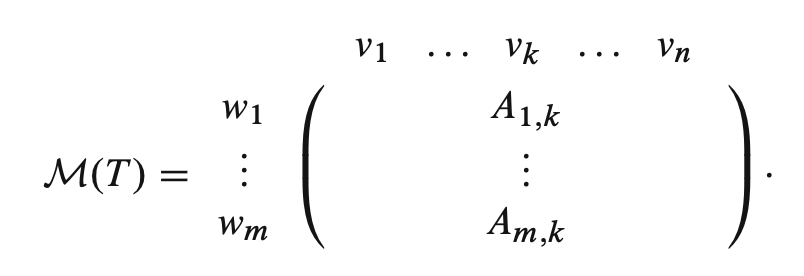
\includegraphics[width=0.8\textwidth]{axler3cmatrix.png}
  \caption{Axler, pg. 71}
  \label{fig:1}
\end{figure}

Only the $k$-th column is included; basically, $T(v_k)$ can be computed by multiplying every
component of $v_k$ by every row of the $k$-th column. That is, the $k$-th column is ``where $v_k$
goes.'' The point is, once bases of $V$ and $W$ are agreed upon, the matrix of $T$, $\mc{M}(T)$,
encodes $T$ without losing information!
\begin{example}
  Suppose $T:\R^2\to \R^3$ is a linear map given uniquely by \[
    T(1,0)=(1,2,7) ~\text{and}~ T(0,1)=(3,5,9)
  .\] Then the matrix $ \mc{M}(T)$ is given by \[
  \begin{pmatrix} 1&3\\2&6\\7&9 \end{pmatrix} 
  .\] 
\end{example}

\subsection{$\mc{L}(V,W)$ as a Vector Space}

Recall that $\mc{L}(V,W)$ denotes the set of linear maps from $V$ to $W$. It turns out that
$\mc{L}(V,W)$ can be given the structure of a vector space! That is, we can define vector addition
and scalar multiplication in such a way to satisfy the properties of a vector space:
\begin{definition}[Addition and Scalar Multiplication in $\mc{L}(V,W)$]{}
  Let $S,T\in \mc{L}(V,W)$, $v\in V$, and $\lambda\in \F $.
  \begin{itemize}
    \item We define $S+T$ to be \[
      (S+T)(v)=S(v)+T(v)
    .\] 
    \item We define $\lambda T$ to be \[
        (\lambda T)(v) = \lambda T(v)
    .\] 
  \end{itemize}
  One can easily check that $S+T$ and $ \lambda T$ are linear maps, and that $\mc{L}(V,W)$ forms a
  vector space (the reader is spared the menial work).
\end{definition}

The additive identity in $\mc{L}(V,W)$ is given by the zero map $0:V\to W$, $0(v)=0$.

Like linear maps, a similar process can be applied for matrices. Let $\F^{m,n}$ denote the set of
$m\times n$ matrices over $ \F$.
\begin{definition}[Addition and Scalar Multiplication in $\F^{m,n}$]{}
  We define addition as component-wise addition; that is, for any $A=(a_{i,j}), B=(b_{i,j})$,
  $A+B=(a_{i,j}+b_{i,j})$. Scalar multiplication is similarly defined: for $A=(a_{i,j}), \lambda A =
  (\lambda a_{i,j})$.
\end{definition}
With these operations, one can easily check that $\F^{m,n}$ is a vector space. Now, we connect
$\mc{L}(V,W)$ to $\F^{m,n}$; intuitively, these two structures should agree.
\begin{proposition}[]{} 
  Given vector spaces $V,W$ over $ \F$ with bases $v_1,\ldots,v_n$ and $w_1,\ldots,w_m$, for any
  $S,T\in \mc{L}(V,W)$, $\lambda\in \F$, we have
  \begin{itemize}
    \item $\mc{M}(S+T)=\mc{M}(S)+\mc{M}(T)$.
    \item $\mc{M}(\lambda T)=\lambda\mc{M}(T)$.
  \end{itemize}
\end{proposition}
The proof should be relatively straightforward; let $A,B$ represent $\mc{M}(S),\ \mc{M}(T)$; then
addition and scalar multiplication in $\mc{L}(V,W)$ should produce the same results as
addition/multiplication in $\F^{m,n}$.

In fact, $\mc{M}(\cdot )$ is itself a map, from $\mc{L}(V,W)$ to $\F^{m,n}$. Indeed, this map is
bijective!
\begin{proposition}[]{}
  Let $V,W$ be finite-dimensional vector spaces over $\F$, and choose bases $v_1,\ldots,v_n$, $
  w_1,\ldots,w_m$. Then \[
    \mc{M}(\cdot ): \mc{L}(V,W)\to \F^{m,n}
  \] is a bijective linear map.
\end{proposition}
\begin{proof}[Proof]
  The previous proposition shows that $\mc{M}(\cdot )$ is linear; to see bijective, for a given
  $A\in \F^{m,n}$, we need to show that there is a unique linear map $T:V\to W$ such that
  $\mc{M}(T)=A$.

  Indeed, by definition of the matrix of a linear map, we wish to show that there exists a unique
  linear map such that, for each $i=1,\ldots,n$, we have \[
    T(v_i)=A_{1,i}w_1+\ldots+A_{m,i}w_m
  .\] But this is true because linear maps are freely and uniquely determined by their operations on
  a basis!
\end{proof}

\begin{remark}
  Recall that an \textit{invertible linear map} or \textit{isomorphism} is one that is bijective.
  Thus this proposition tells us that there is an isomorphism between $\mc{L}(V,W)$ and $\F^{m,n}$.
\end{remark}

\subsection{Composition of Linear Maps and Products of Matrices}

Usually, vector multiplication doesn't make sense, but for some pairs of linear maps, a meaningful
product exists.
\begin{definition}[Product of Linear Maps]{}
  If $T\in \mc{L}(U,V)$, and $S\in \mc{L}(V,W)$, then the \textbf{product} $ST\in \mc{L}(U,W)$ is
  defined by \[
    (ST)(u)=S\circ T(u)=S(T(u))
  \] for $u\in U.$
\end{definition}
In other words, $ST$ is just the usual composition $S\circ T$ of two functions. One can easily
verify that $ST\in \mc{L}(U,W)$ is a linear map from $U$ to $W$.

\begin{definition}[Linear Operators]{}
  A linear map $T:V\to V$ from a vector space to itself is called a \textbf{linear operator}.
\end{definition}
\begin{proposition}[]{}
  The composition of linear maps is associative and distributive, an identity $I$ exists. However,
  it is \textbf{not necessarily} commutative; that is, $ST\neq TS$. Moreover, $ST=0$ does
  \textbf{not} imply that $S=0$ or $T=0$.
\end{proposition}

We now have products of linear maps; but what is the analogy for matrices?

\begin{definition}[Matrix Multiplication]{}
  Suppose $A\in \F^{m,n}$ is an $m\times n$ matrix, and $C\in \F^{n,p}$ is an $n\times p$ matrix.
  Then $AC\in \F^{m,p}$ is defined by the $m\times p$ matrix with $AC_{j,k}$-th entry given by:  \[
    (AC)_{j,k}=\sum_{r=1}^{n} A_{j,r}C_{r,k}
  .\] In other words, the entry in row $j$, column $k$, of $AC$ is computed by multiplying piecewise
  row $j$ of $A$ and row $k$ of $C$.
\end{definition}

Note that in order to multiply, the inner values (e.g. $m\times n$ and $n\times p$) must agree! That
is, $3\times 2$ and $2\times 4$ would work, but $3\times 1$ and $3\times 2$ wouldn't.
\begin{example}
  Here we multiply a $3\times 2$ and $2\times 4$ matrix: \[
    \begin{pmatrix} 1&2\\3&4\\5&6 \end{pmatrix} \begin{pmatrix} 6&5&4&3 \\2&1&0&-1\end{pmatrix}
    =\begin{pmatrix} 10&7&4&1\\26&19&12&5\\42&31&20&9 \end{pmatrix}
  .\] 
\end{example} 

\begin{proposition}[]{}
  Suppose $T:U\to V$, $S:V\to W$ are linear maps with fixed bases. Then \[
    \mc{M}(ST)=\mc{M}(S)\mc{M}(T)
  .\] 
\end{proposition}
This proof is the result of tedious computation; see Axler p.74.


\section{Invertibility and Isomorphic Vector Spaces}

\subsection{Invertible Linear Maps}

We start by looking at invertible linear maps, and inverses in the context of linear maps.

\begin{definition}[Invertible, Inverse]{}
  A linear map $T\in \mc{L}(V,W)$ is called \textbf{invertible} if there exists a linear map $S\in
  \mc{L}(W,V)$ such that $ST=I_V$, and $TS=I_W$. $S\in \mc{L}(W,V)$ is called the \textbf{inverse}
  of $T$.
\end{definition}

\begin{proposition}[Inverse is Unique]{}
  an invertible linear map is unique.
\end{proposition}
\begin{proof}[Proof]
  Suppose $T\in \mc{L}(V,W)$ is invertible, and $S_1,S_2$ are inverses of $T$. Then \[
    S_1=S_1I=S_1(TS_2)=(S_1T)S_2=IS_2=S_2
  .\] 
\end{proof}

Thus, we can denote the inverse of a map $T\in \mc{L}(V,W)$ uniquely by $T^{-1}\in \mc{L}(W,V)$. It
turns out that invertibility is equivalent to bijectivity:
\begin{proposition}[]{}
  A linear map is invertible if and only if it is bijective.
\end{proposition}
\begin{proof}[Proof]
  We first sketch a proof, then proceed formally.

  In order to be an inverse of $T \in \mc{L}(V,W)$, an inverse $T ^{-1}\in \mc{L}(W,V)$ must
  ``undo'' $T$, and vice versa; that is, for any $v\in V$, $T^{-1}T(v)=v$, and for any $w\in W$,
  $TT^{-1}(w)=w$. Thus, it is clear that
  \begin{itemize}
    \item $T$ must be injective: if it is not, then at least two elements in $V$ map to the same
      element in $w$, so how is a $T^{-1}$ supposed to ``undo'' this operation?
    \item $T$ must be surjective: if it is not, then some element in $w\in W$ is not mapped to by
      $T$; that is, no such $v\in V$ exists such that $T(v)=w$. Then how is $T$ supposed to ``undo''
      $w$, if it never maps to $w$?
  \end{itemize}

  Now, we proceed formally. Suppose $T$ is invertible; that is, some $T^{-1}\in \mc{L}(W,V)$ has the
  property $TT^{-1}=T^{-1}T=I$. Suppose $T(u)=T(v)$ for some $u,v\in V$. Then \[
    u=T^{-1}T(u)=T^{-1}T(v)=v
  ,\] and so $T$ is injective. Now, let $w$ be any element in $W$. Then $w=T(T^{-1}(w))$, and so
  $w\in \range{T}$. Thus $\range{T}=W$, and so $T$ is surjective, and thus a bijection.\\

  Conversely, suppose $T\in \mc{L}(V,W)$ is a bijection. Then for every $w\in W$, there exists a
  unique $v\in V$ such that $T(v)=w$. Define $S\in \mc{L}(W,V)$ as the function that sends every
  $w$ back to its original $v$; that is, since $w=T(v)$, we have $S(w)=S(T(v))=v$. Clearly, $T\circ
  S$ is the identity map $I_W$. To show that $S\circ T=I_V$, consider any $v\in V$. Then \[
    T(S\circ T(v))=(T\circ S)T(v)=I_WT(v)=T(v)
  .\] Then $T(S\circ T(v))=T(v)$; but since $T$ is an injection, we have $S\circ T(v)=v$, and so
  $S\circ T=I_V$. Thus $S=T^{-1}$.

  It remains to prove that $S$ is a linear map. In order to satisfy linear map properties, we need
  to show that \[
    S(a_1w_1+a_2w_2)=a_1S(w_1)+a_2S(w_2)
  .\] Since $T$ is injective, we really only need to show that \[
    T(S(a_1w_1+a_2w_2))=T(a_1S(w_1)+a_2S(w_2))
  .\] Indeed, we have
  \begin{align*}
    T(S(a_1w_1+a_2w_2))&= a_1w_1+a_2w_2 \\
                       &= a_1T(S(w_1))+a_2T(S(w_2)) \\
                       &= T(a_1S(w_1))+T(a_2S(w_2)) \\
                       &= T(a_1S(w1)+a_2S(w_2))
  .\end{align*} Hence $S$ is a linear map.
\end{proof}

\subsection{Isomorphic Vector Spaces}

From this, we get the sense that if an invertible linear map exists between two vector spaces, then
they are essentially the same; they differ only in the names of their elements.

\begin{definition}[Isomorphic, Isomorphism]{}
  An \textbf{isomorphism} is an invertible linear map. Two vector spaces $V,W$ are
  \textbf{isomorphic} if there is an isomorphism between the two; we write $V\cong W$.
\end{definition}

Isomorphic vector spaces are really the same name; one can picture any element $v\in V$ as being
``relabeled'' as $T(v)\in W$. Thus, a natural proposition follows.
\begin{theorem}[Dimension of Isomorphic Vector Spaces]{}
  Let $V,W$ be finite-dimensional vector spaces. Then $V\cong W$ if and only if $\dim V = \dim W$.
\end{theorem}
\begin{proof}[Proof]
  First, suppose $V\cong W$. Then there exists an isomorphism $T\in \mc{L}(V,W)$; moreover, $T$ is
  bijective. Thus $ \Null{T}=0$, and $\range T = W$, and so $\dim\Null T = 0,\ \dim \range T
  =\dim W$. Then \[
    \dim V = \dim\Null T + \dim\range T
  \] becomes $\dim V = \dim W$, as required.

  Conversely, suppose $\dim V = \dim W$. Let $v_1,\ldots,v_n$ be a basis for $V$, and let $
   w_1,\ldots,w_n$ be a basis for $W$. Let $T\in \mc{L}(V,W)$ be defined as \[
     T(c_1v_1+\ldots+c_nv_n)=c_1w_1+\ldots+c_nw_n
   .\] Then $T$ is a well-defined, unique linear map, since $v_1,\ldots,v_n$ is a basis. $T$ is
   surjective, since $w_1,\ldots,w_n$ spans $W$; moreover, $ \Null T=\{ 0 \}$, since
   $w_1,\ldots,w_n$ is linearly independent, so $ c_1w_1+\ldots+c_nw_n=0$ iff $c_i=0$
   (alternatively, one can use the rank-nullity theorem and the fact that $\dim\range T = \dim W =
   \dim V$, so $\dim\Null T$ is necessarily $0$). Thus $T$ is injective, and so $T$ is an
   isomorphism. Hence $V\cong W$, as required.
\end{proof}

From this, we get that any finite-dimensional vector space $V$ with dimension $n$ is actually
isomorphic to $\F^{n}$! But then, why don't we only study the vector spaces $\F^{n}$, if they're
really the same as any other vector space with dimension $n$? Studying vector spaces abstractly is
extremely useful; for example, the polynomial space of dimension 15 is quite useful in physics.

Our discussion about dimensions and isomorphism lead us to the following proposition:
\begin{proposition}[]{}
  Suppose $V,W$ are finite-dimensional vector spaces with $ \dim V = \dim W$, and let $T\in
  \mc{L}(V,W)$ be a linear map. The following are equivalent:
  \begin{enumerate}
    \item $T$ is invertible/bijective.
    \item $T$ is injective.
    \item $T$ is surjective.
  \end{enumerate}
\end{proposition}

\begin{proof}[Proof]
  Let $n=\dim V = \dim W$. Then $n=\dim V=\dim\Null T + \dim\range T$. So $\dim\Null T=0 \iff
  \dim\range T=n\iff \dim\Null T=0 ~\text{AND}~\dim\range T=n$. In other words, $T$ is injective iff
  $T$ is surjective iff $T$ is bijective.
\end{proof}













\end{document}
